\documentclass{lug}

\title{Penguinitis}
\subtitle{\emph{aka} Why we're addicted to Linux}
\author{Jack Rosenthal}

\newcommand{\tuxdistroheader}{%
    \hskip 0cm plus 1filll
    \raisebox{-5pt}{
\includegraphics[height=18pt]{graphics/tux_header_icon}}
    \textbf{Distros}
}

\usepackage{tcolorbox}

\begin{document}

\begin{frame}
    \frametitle{What is Linux?}

    \begin{columns}
        \begin{column}{0.7\textwidth}
        \begin{itemize}[<+->]
            \setlength\itemsep{1em}
            \item Linux is an UNIX-like \textbf{operating system kernel},
                meaning it only provides the core components of the OS
            \item Linux is free and open source software written by developers
                across the world
            \item Linux can be used as a desktop OS, on servers, and Linux even
                powers Android
            \item Linux distributions (\emph{distros}) are complete operating
                systems created by bundling Linux with other software
        \end{itemize}
        \end{column}

        \begin{column}{0.3\textwidth}
            
\includegraphics[width=\textwidth]{graphics/TuxFlat}
        \end{column}
    \end{columns}
\end{frame}

\begin{frame}
    \frametitle{Who develops Linux?}

    \begin{figure}
        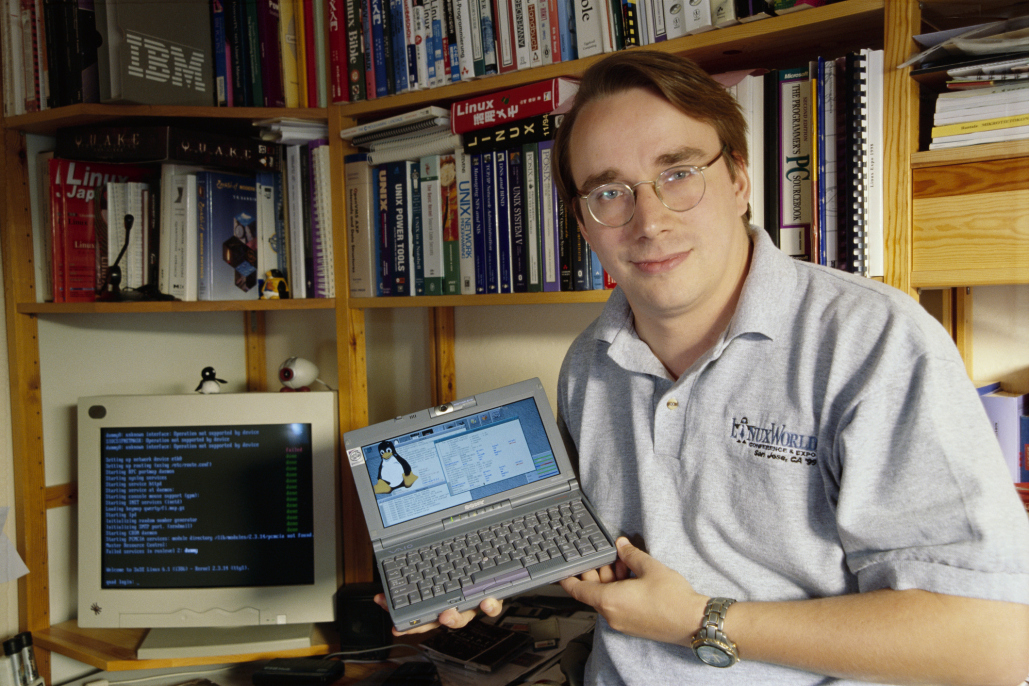
\includegraphics[width=0.75\textwidth]{graphics/torvaldslinux}

        \bigskip

        \begin{minipage}{0.75\textwidth}
            \centering
            \small
        \emph{Linus Torvalds} (pictured above) started the Linux project, and although
        he has only written 2\% of the code, he has written the most of anyone
        alone.
        \end{minipage}
    \end{figure}

\end{frame}

\begin{frame}
    \frametitle{The UNIX Philosophy}

    \begin{columns}
        \begin{column}{0.8\textwidth}
    UNIX-like operating systems have been traditionally \emph{written by
    programmers, made for programmers}. This means it is easy to
    programmatically work on data.
        \end{column}
        \begin{column}{0.2\textwidth}
            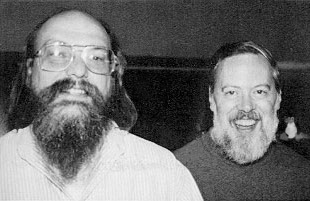
\includegraphics[width=\textwidth]{graphics/ken_dmr}
        \end{column}
    \end{columns}

    \bigskip

    \begin{tcolorbox}[size=fbox,sharp corners=all]
        \small
    \begin{enumerate}
        \setlength\itemsep{2pt}
        \item \small Write programs which do one thing, and one thing well
        \item \small The output of a program should become the input of another
    \end{enumerate}
    \end{tcolorbox}

    \bigskip

    {%
        \bfseries
        \only<1>{$\,$}
        \only<2>{Download a file from a URL and write to terminal}
        \only<3>{Download a file from a URL while uncompressing it}
        \only<4>{Do all that while writing to a disk}
    }

    \medskip

    \visible<2->{\texttt{curl http://site/d.img.gz\visible<3->{\ |
    zcat\visible<4->{\ | dd of=/dev/sdb}}}}
\end{frame}

\begin{frame}
    \frametitle{Package Management}
    \vglue-20pt
    \begin{columns}[T]
        \begin{column}{0.5\textwidth}
            \begin{center}
                
\includegraphics[height=3em]{graphics/mswindows}\par
                \textbf{The Windows Way}
            \end{center}
            \vglue-10pt
            \small
            \begin{itemize}
                \item Users get software by visiting a website and downloading
                    the installer program
                \item Developers have to write update managers
                \item Developers have to write an uninstaller program
                \item Dependency resolution is done by sketchy hacks in the
                    installer program
            \end{itemize}
        \end{column}
        \begin{column}{0.5\textwidth}
            \begin{center}
                
\includegraphics[height=3em]{graphics/TuxFlat}\par
                \textbf{The Linux Way}
            \end{center}
            \vglue-10pt
            \small
            \begin{itemize}
                \item Distributions include a \textbf{package manager}, a
                    program which is responsible for:
                    \begin{itemize}
                        \item software installation
                        \item dependency resolution
                        \item software updates
                        \item software removal
                    \end{itemize}
            \end{itemize}
        \end{column}
    \end{columns}
\end{frame}



\begin{frame}
    \frametitle{Linux is Ultra Customizable}

    Because Linux is just a kernel, so many software packages exist to run on
    top of it. You get the choice of these packages to make the desktop just
    how you like it.

    \bigskip


    \begin{columns}
        \begin{column}{0.3\textwidth}
            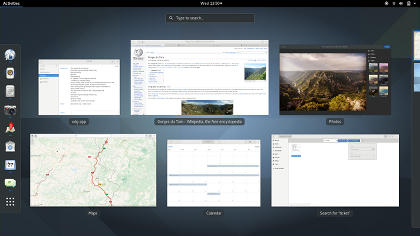
\includegraphics[width=\textwidth]{graphics/gnome} \par
            \vspace*{4pt}
            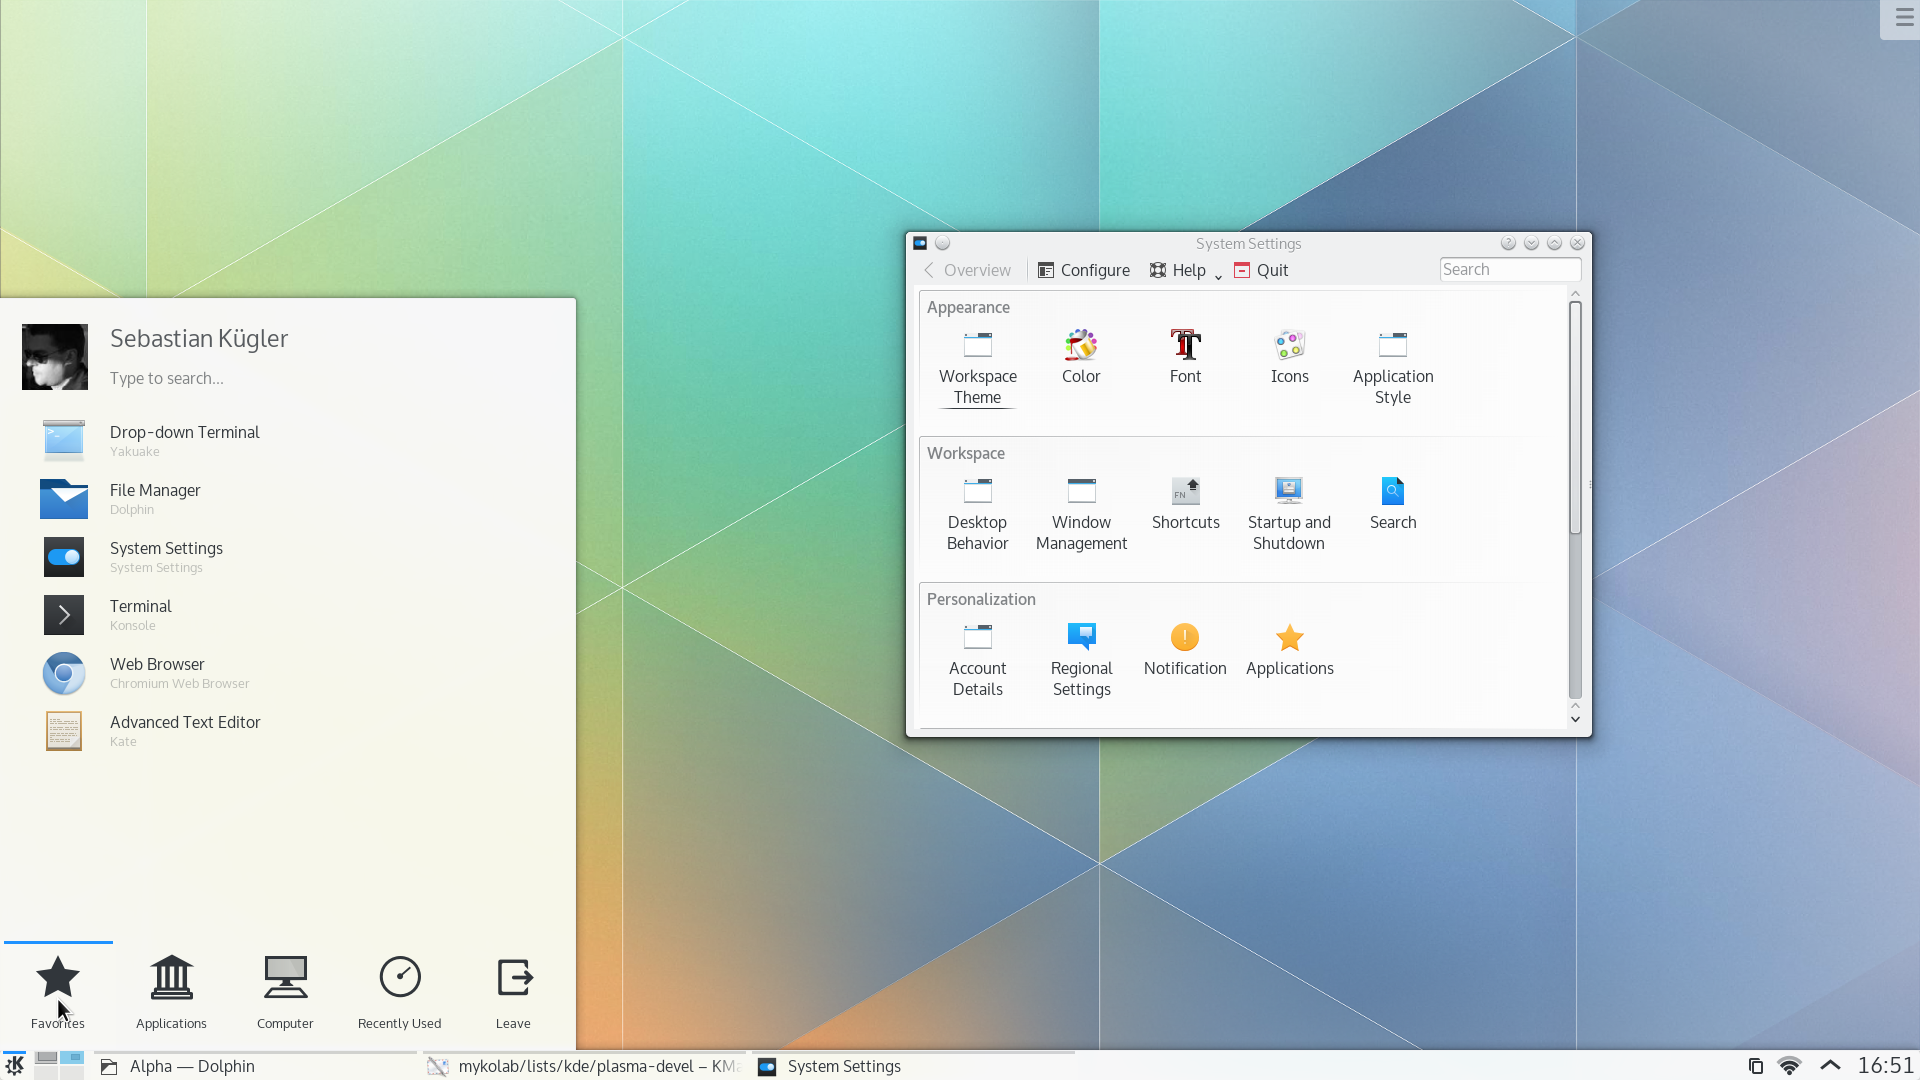
\includegraphics[width=\textwidth]{graphics/kde} \par
        \end{column}
        \begin{column}{0.3\textwidth}
            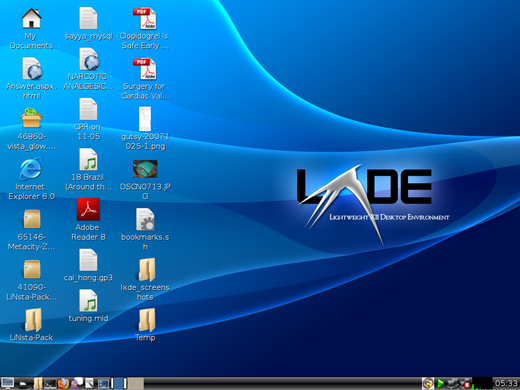
\includegraphics[width=\textwidth]{graphics/lxde} \par
            \vspace*{4pt}
            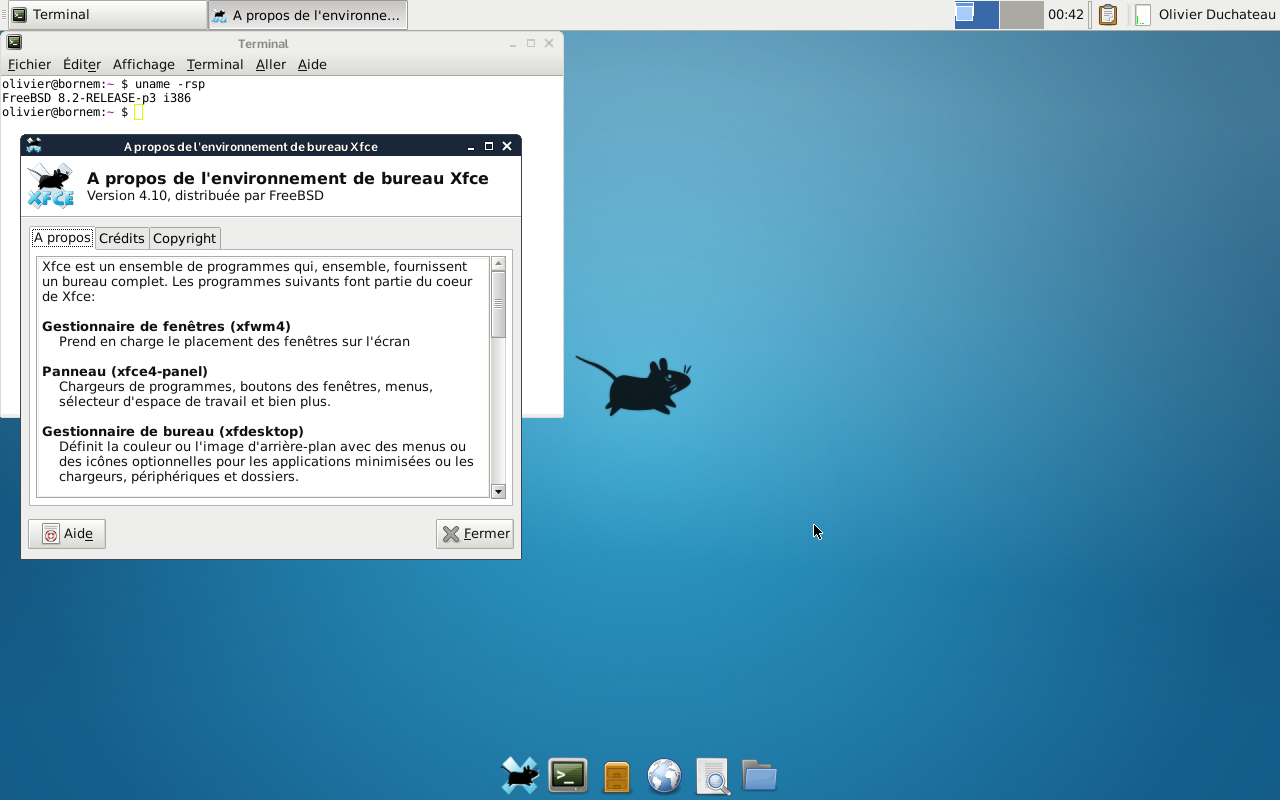
\includegraphics[width=\textwidth]{graphics/xfce} \par
        \end{column}
        \begin{column}{0.3\textwidth}
            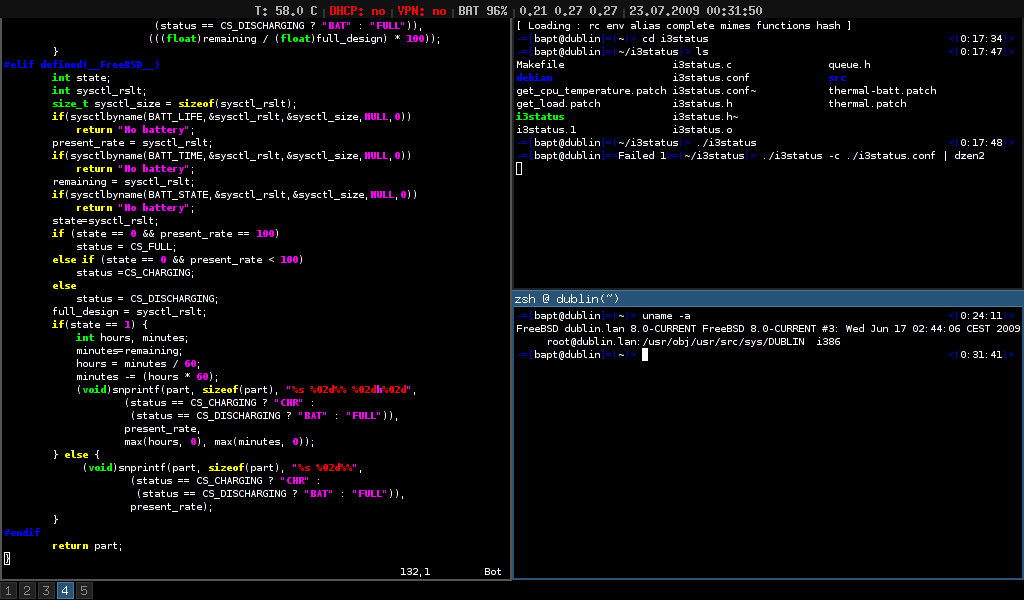
\includegraphics[width=\textwidth]{graphics/i3} \par
            \vspace*{4pt}
            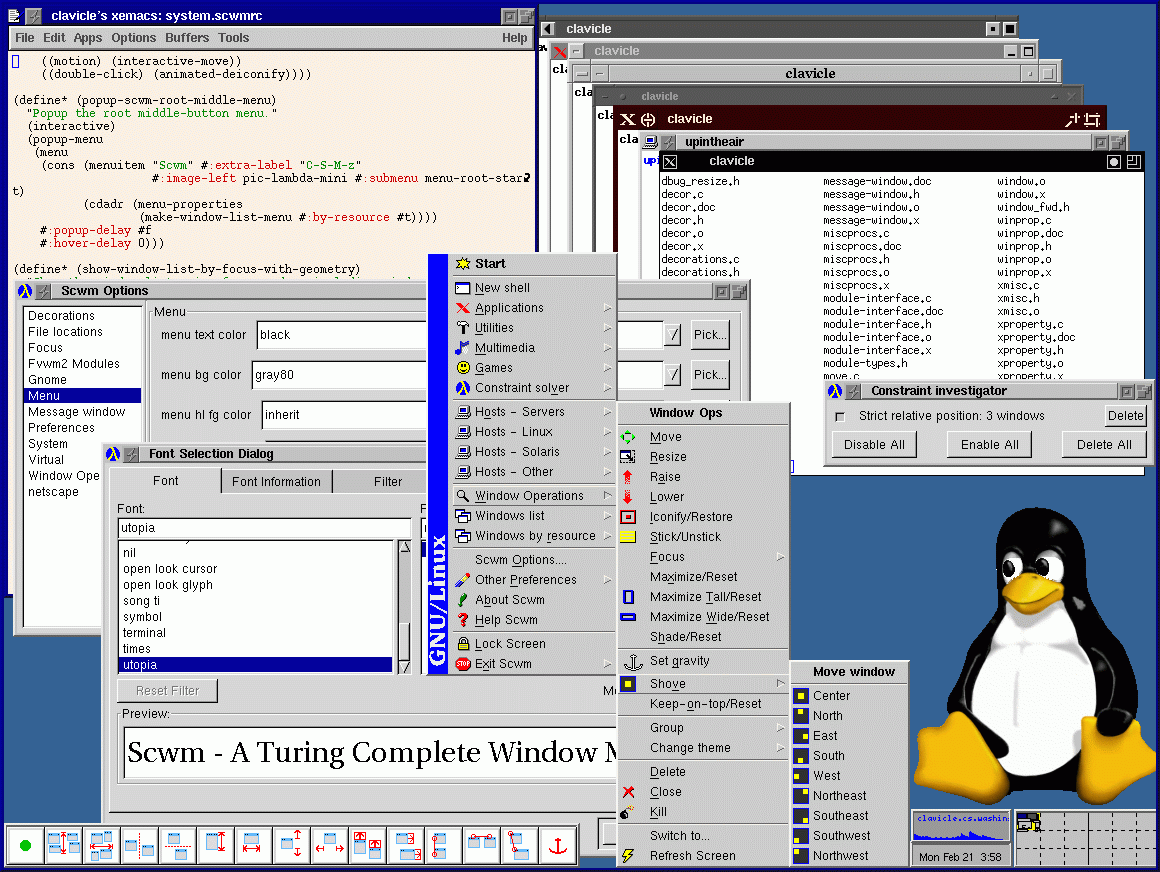
\includegraphics[width=\textwidth]{graphics/scwm} \par
        \end{column}
    \end{columns}
\end{frame}

\begin{frame}
    \frametitle{Debian \tuxdistroheader}
    \begin{columns}
        \begin{column}{0.7\textwidth}
        \begin{itemize}[<+->]
            \setlength\itemsep{1em}
            \item Started in 1993, an old, yet reliable, distribution
            \item Installation images with GNOME, Cinnamon, KDE, LXDE,
                MATE, and XFCE
            \item Features the \texttt{apt} package manager
        \end{itemize}
        \end{column}

        \begin{column}{0.3\textwidth}
            
\includegraphics[width=\textwidth]{graphics/debian}
        \end{column}
    \end{columns}
\end{frame}

\begin{frame}
    \frametitle{Ubuntu \tuxdistroheader}
    \begin{columns}
        \begin{column}{0.7\textwidth}
        \begin{itemize}[<+->]
            \setlength\itemsep{1em}
            \item A Debian based distribution started in 2004
            \item Many flavors including Kubuntu, Lubuntu, Xubuntu, Ubuntu
                GNOME and more
            \item Very popular and has a large community
            \item Features the \texttt{apt} package manager, as well as a
                ``Software Manager'' GUI
        \end{itemize}
        \end{column}

        \begin{column}{0.3\textwidth}
            
\includegraphics[width=\textwidth]{graphics/ubuntu}
        \end{column}
    \end{columns}
\end{frame}

\begin{frame}
    \frametitle{Linux Mint \tuxdistroheader}
    \begin{columns}
        \begin{column}{0.7\textwidth}
        \begin{itemize}[<+->]
            \setlength\itemsep{1em}
            \item A Ubuntu based distribution started in 2006
            \item Comes with an interface that may be very familiar to previous
                users of Microsoft Windows, and because of this, many people
                call it beginner friendly
            \item Basically another Ubuntu
        \end{itemize}
        \end{column}

        \begin{column}{0.3\textwidth}
            
\includegraphics[width=\textwidth]{graphics/mint}
        \end{column}
    \end{columns}
\end{frame}

\begin{frame}
    \frametitle{Fedora \tuxdistroheader}
    \begin{columns}
        \begin{column}{0.7\textwidth}
        \begin{itemize}[<+->]
            \setlength\itemsep{1em}
            \item Started in 2003 after the discontinuation of Red Hat Linux
            \item Main distribution features GNOME, although there are
                \emph{spins} of other desktop environments
            \item Includes power user tools like GNOME Boxes and Docker support
                out of the box
            \item Easy for beginners
            \item Features the excellent \texttt{dnf} package manager
        \end{itemize}
        \end{column}

        \begin{column}{0.3\textwidth}
            
\includegraphics[width=\textwidth]{graphics/fedora}
        \end{column}
    \end{columns}
\end{frame}

\begin{frame}
    \frametitle{Arch Linux \tuxdistroheader}
    \begin{columns}
        \begin{column}{0.7\textwidth}
        \begin{itemize}[<+->]
            \setlength\itemsep{1em}
            \item Started in 2002 and there hasn't been a new version released
                since
            \item I'm not joking\dots\ Arch Linux is a rolling release. Updating
                your system through \texttt{pacman} brings you to the latest
            \item Comes with basically nothing out of the box, it's up to you
                to install the software you want to use
            \item Software packages are usually bleeding edge
            \item Very helpful and kind community
        \end{itemize}
        \end{column}

        \begin{column}{0.3\textwidth}
            
\includegraphics[width=\textwidth]{graphics/arch}
        \end{column}
    \end{columns}
\end{frame}

\begin{frame}
    \frametitle{Choosing a Distro}

    \begin{columns}
        \begin{column}{0.7\textwidth}
        \begin{itemize}[<+->]
            \setlength\itemsep{1em}
            \item Do your own research to see which distro appeals to you the
                most
            \item You may have to install a few different distros and try them
                out
            \item Most Linux distros have a \emph{Live CD} image that allows
                you to try the full desktop from a CD or USB drive before installing
        \end{itemize}
        \end{column}

        \begin{column}{0.3\textwidth}
            
\includegraphics[width=\textwidth]{graphics/tux_flag}
        \end{column}
    \end{columns}
\end{frame}

\begin{frame}
    \frametitle{So do you have Penguinitis?}
    \centering
    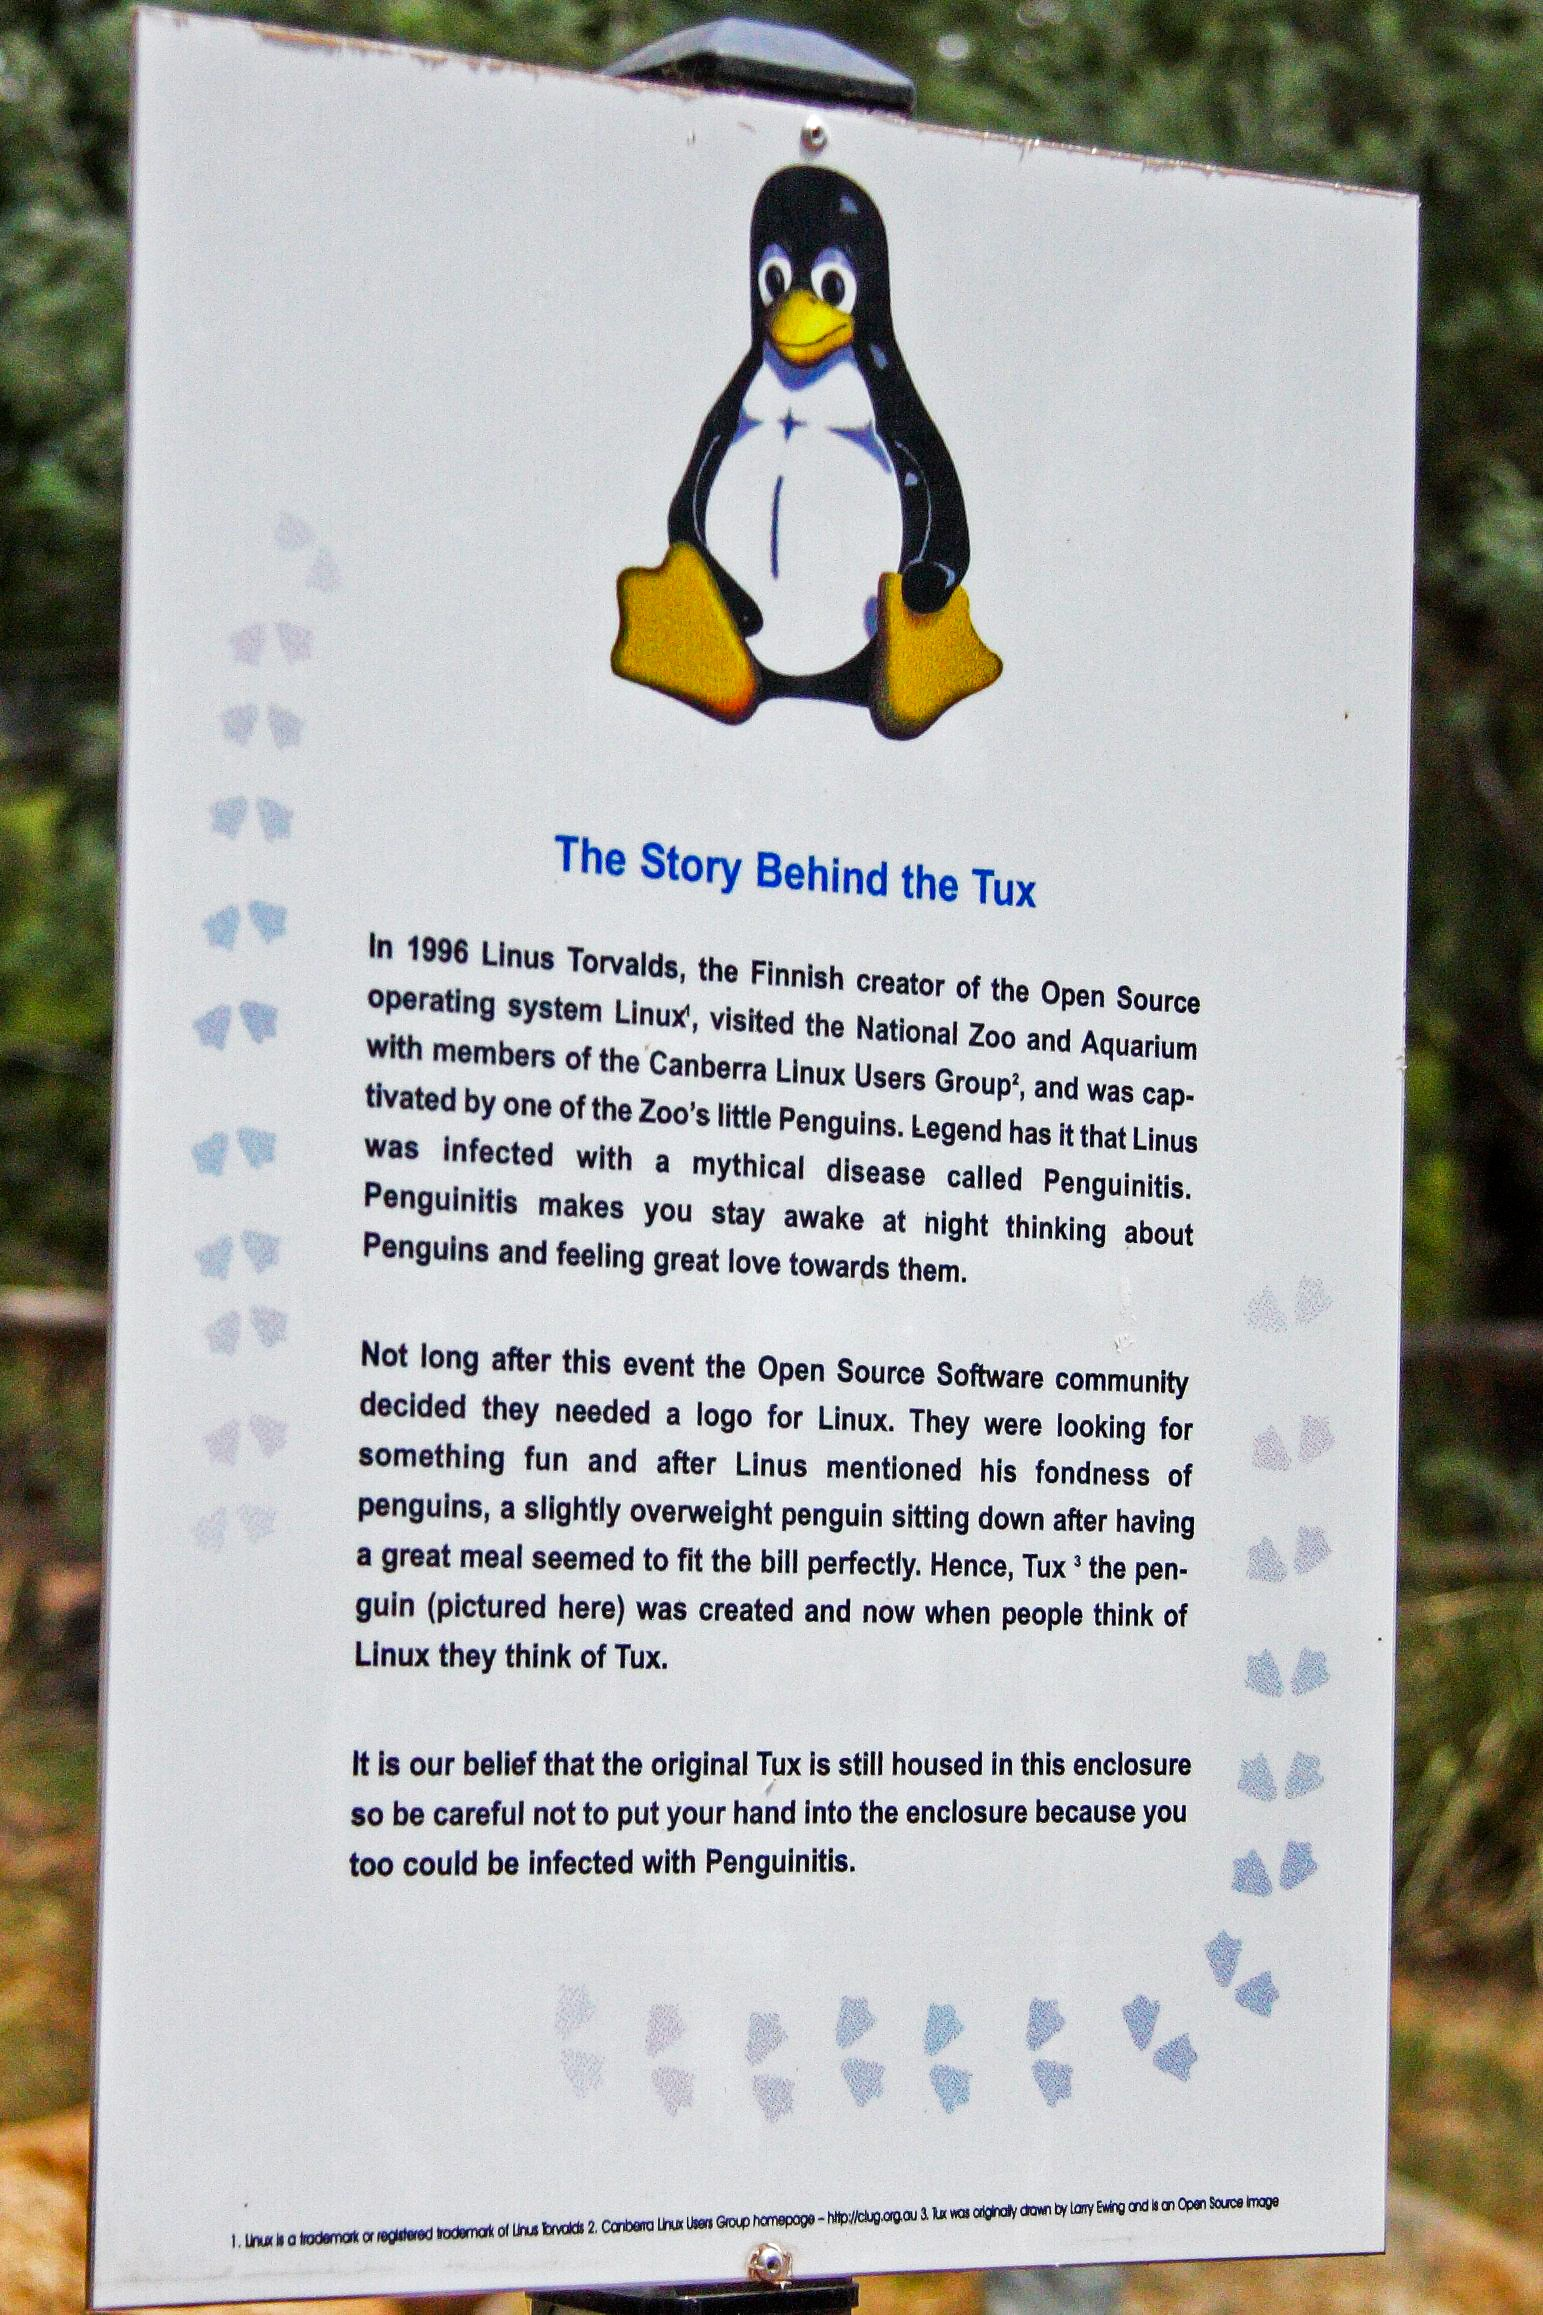
\includegraphics[height=\paperheight-4em]{graphics/penguinitis}
\end{frame}

\end{document}
